\section{Experimental results}

\subsection{Dataset preprocessing}

The dataset in use is the Illinois Bulk Dataset, that contains 
183146 cases with 194366 judges opinions. 

The first step of the preprocessing is to merge the opinions about a 
case into one, obtaining a single document for each dataset entry.  
Then, each document goes through a text cleaning and tokenization phase, 
where the first part is done with the help of regular expressions, 
while the second uses Spacy to obtain a list of terms.

\subsection{Word of interest expansion}

The project started with a collection of relevant words for three categories, 
namely weapons, narcotics and investigations. The idea is to preserve these words
in each preprocessing phase, especially when filtering out words 
that do not meet a required frequency in the dataset. 
To have a better set of interesting words to keep we opted to expand them 
using pre-trained word embeddings, the \emph{GoogleNews} models.
The process consists of finding similar words for each word 
of interest, checking that these words are in the dataset, 
with a manual final review to remove unnecessary or wrong words.

\subsection{Topic modelling}

To have an overview of the topics discussed on the dataset a Latent 
Dirichlet Allocation model is trained on the tokenized texts.
One of the key parameters of such a model is the number of topics, and, 
given the fact that cases could potentially talk about anything, an 
\emph{Halving search} is performed to find a good value.

We opt for an halving search since the number of topics could be anything, 
we fixed a range between ten and thirty and training each model 
to then evaluate results would take a huge amount of time. Halving search 
mitigates the problem, as it trains firstly on smaller datasets, select 
the best models, and retrain on bigger slices of data until a final model 
is found. This methodology can be ten times faster then grid search. 
The selection criterium for the search is the Log Likelihood of each model.
The search revealed that the optimal number of topics is 14. An overview of the found topics 
can be seen on Figure \vref{figt1}.

\begin{figure}
  \begin{center}
    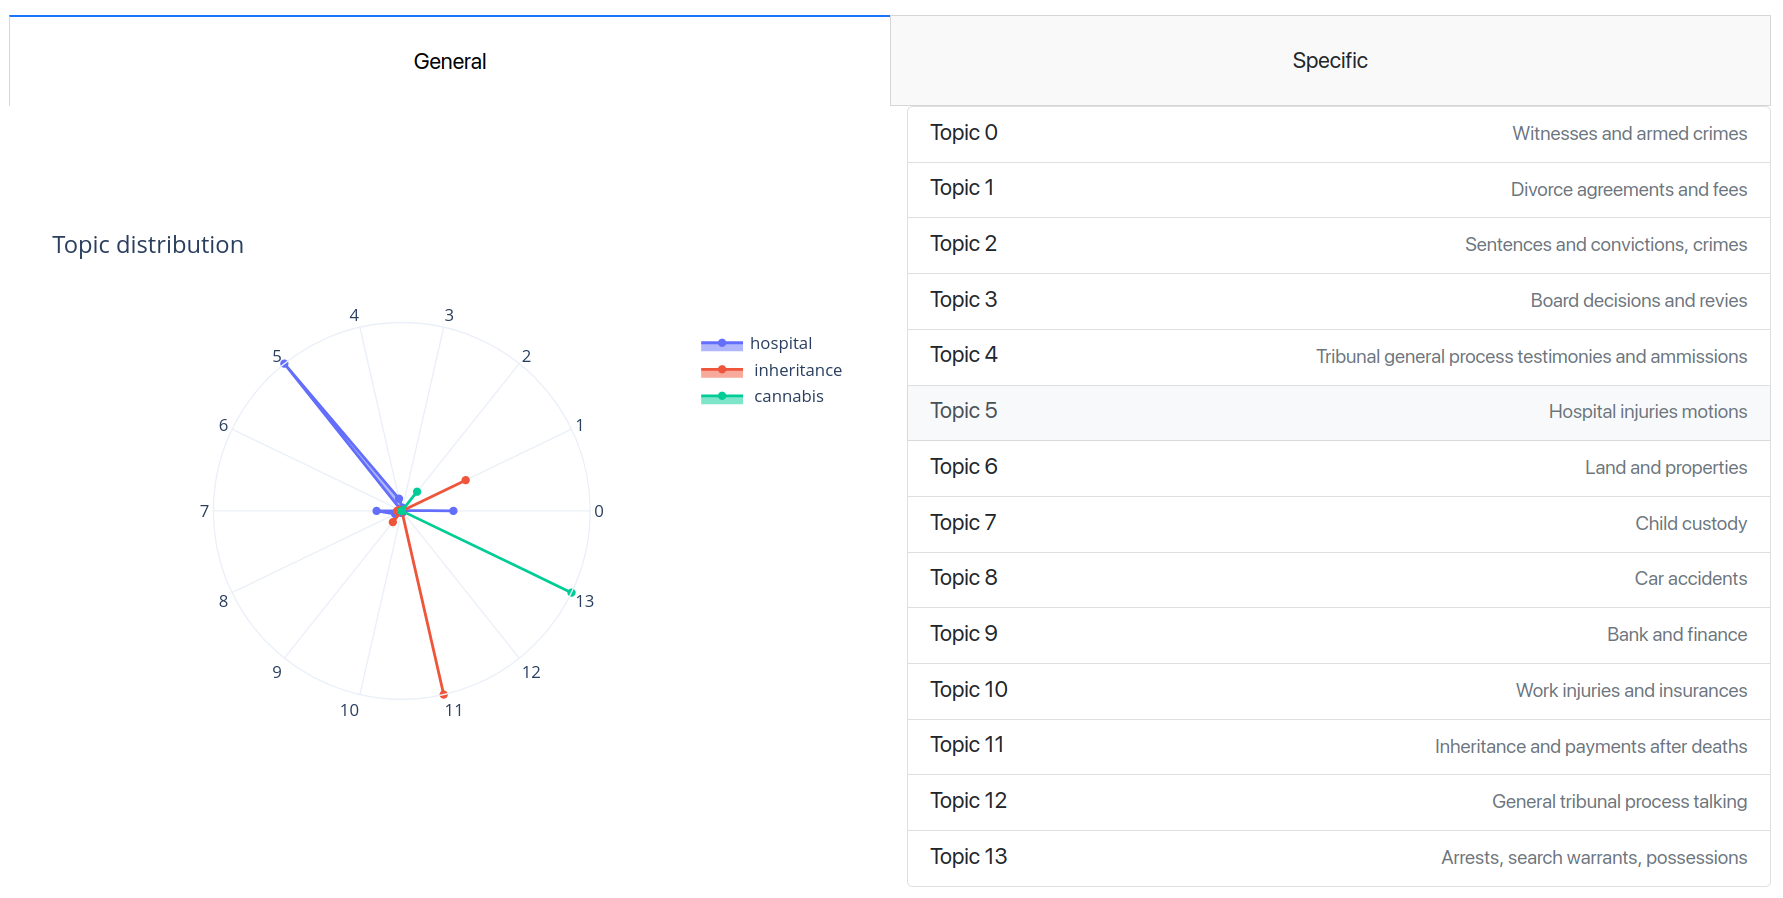
\includegraphics[width=\textwidth]{images/topic1.png}
    \caption{Generic topic distribution for the words hospital, inheritance and cannabis} \label{figt1}
  \end{center}
\end{figure}

The results are promising but the words of interest, namely a collection 
of narcotics, investigation and weapons terms, are merged together in a few topics.

To solve the issue we decide to run topic modelling on a subset of the previous 
topics with the same technique as before. The result is similar, we find again 14 topics, 
but this time they are much more specific, an example of specific topic distribution can be seen on Figure \vref{figt2}, with an in depth topic analysis on Figure \vref{figt3} 
\begin{figure}
  \begin{center}
    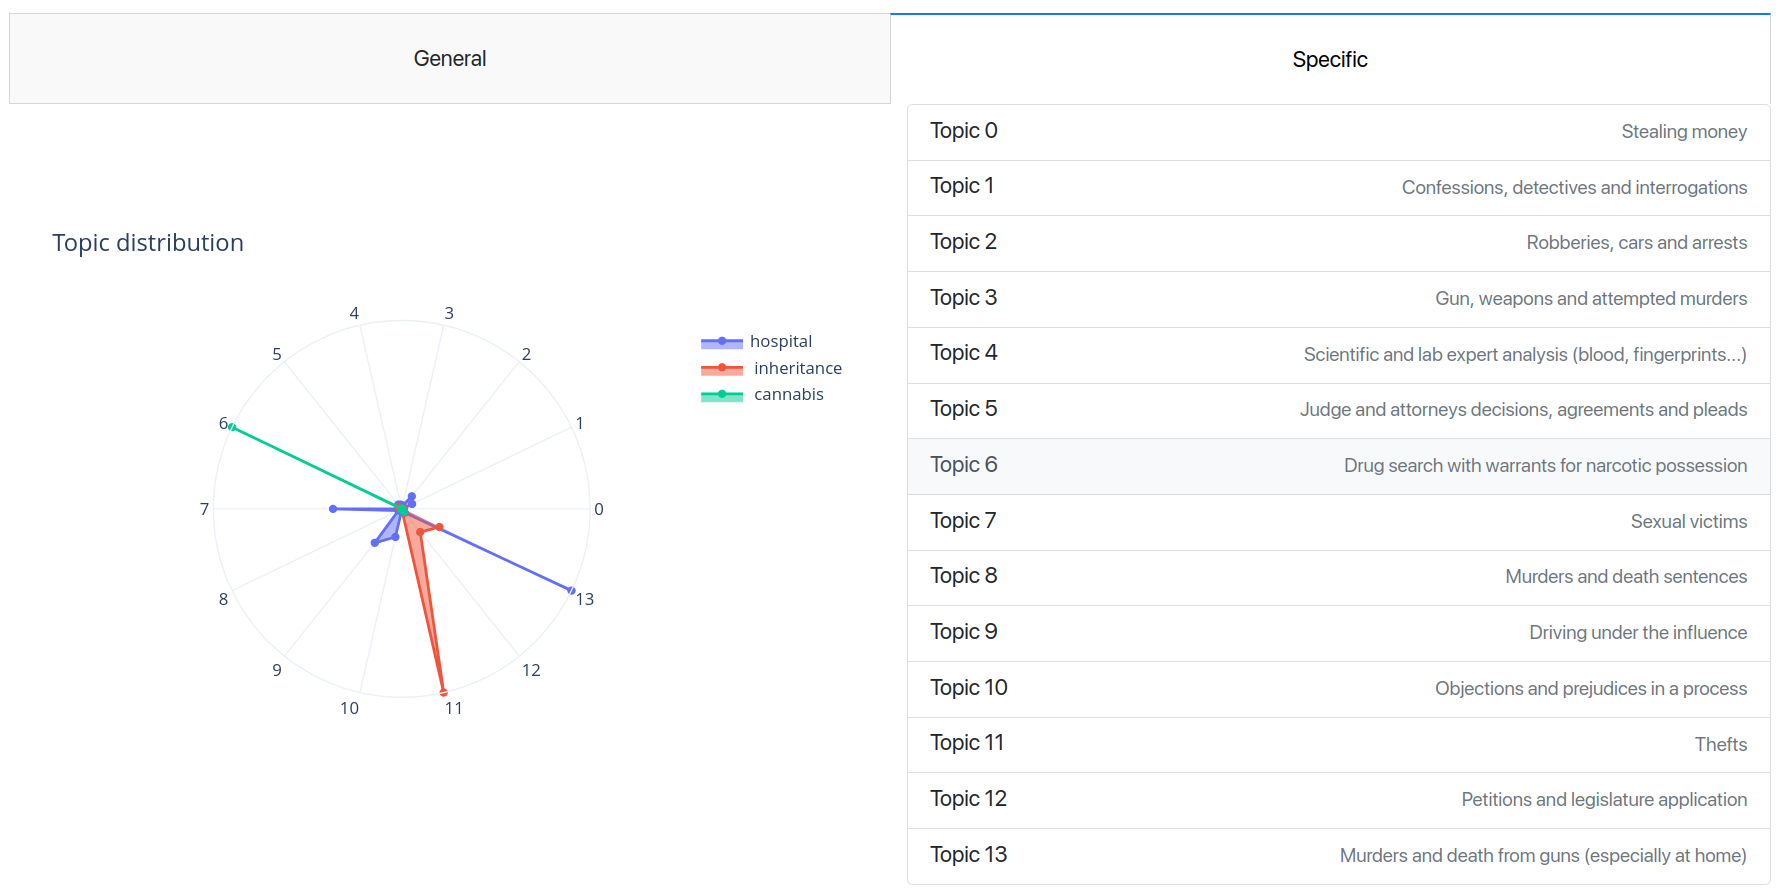
\includegraphics[width=\textwidth]{images/topic2.png}
    \caption{Specific topic distribution for the words hospital, inheritance and cannabis} \label{figt2}
  \end{center}
\end{figure}
\begin{figure}
  \begin{center}
    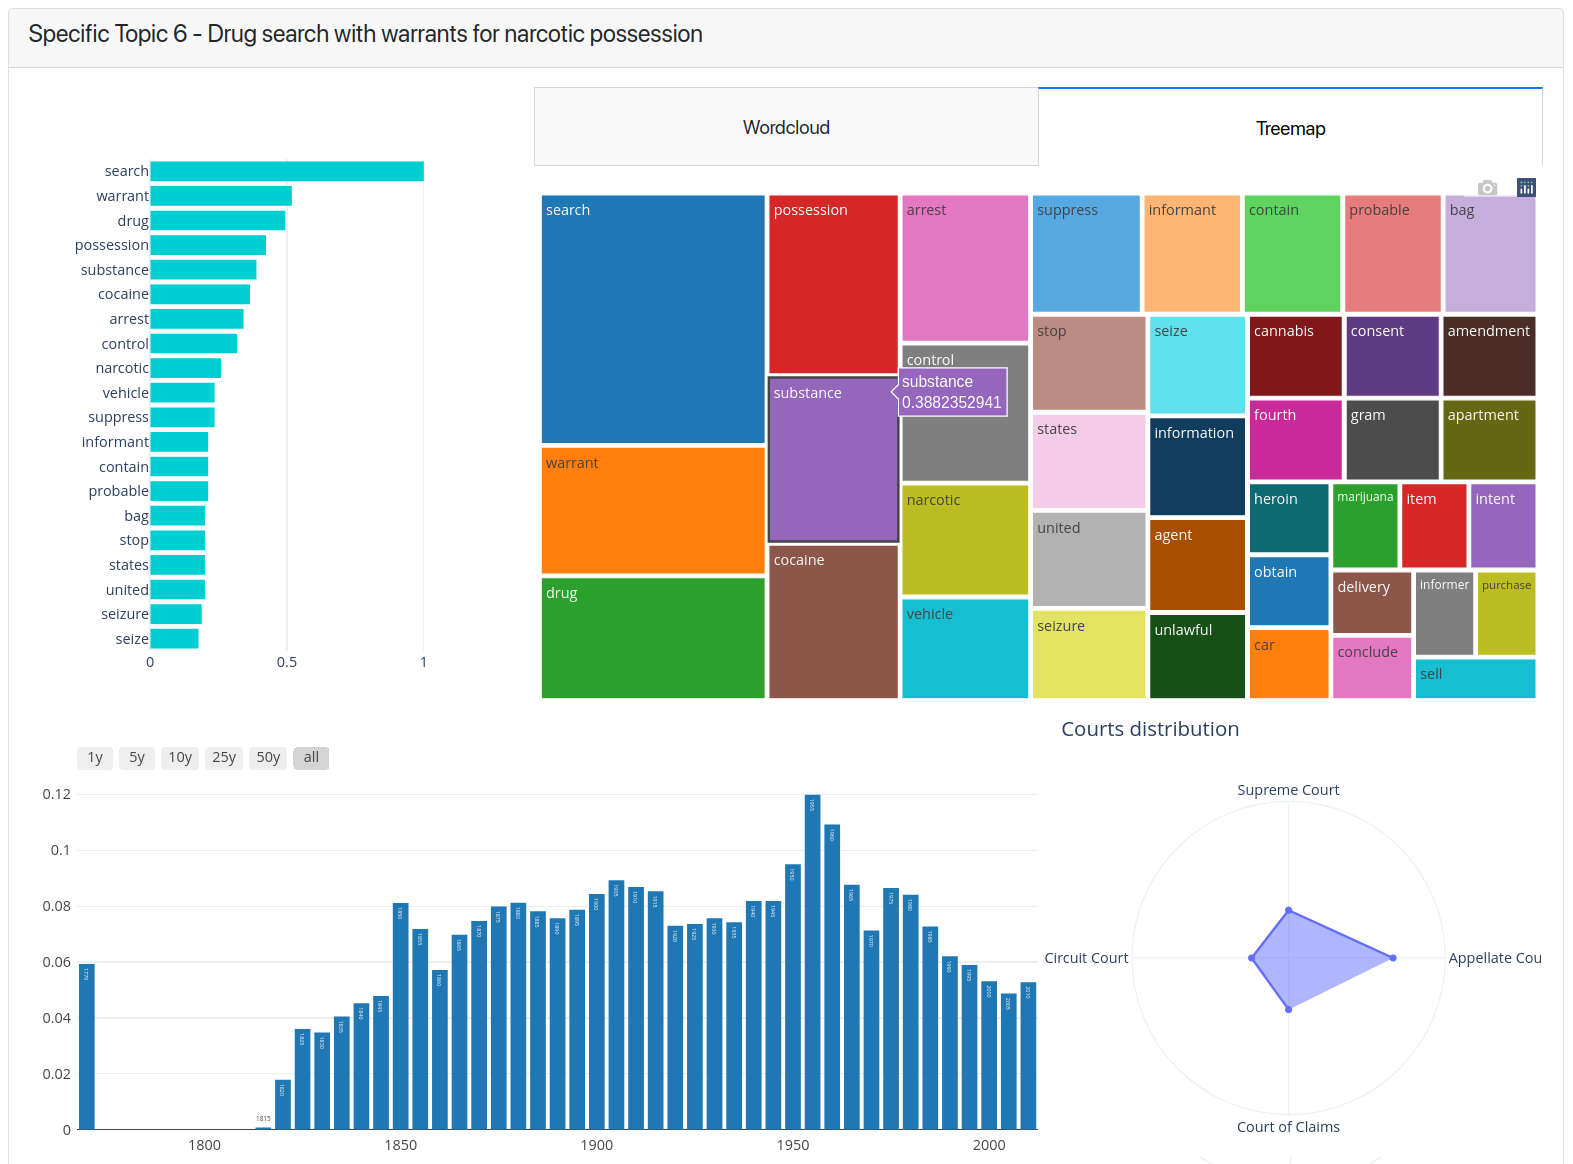
\includegraphics[width=\textwidth]{images/topic3.png}
    \caption{Detailed topic analysis for the search warrant specific topic.} \label{figt3}
  \end{center}
\end{figure}

As stated on Subsection \vref{res-med}, the first idea was to guide the topic modelling
process to find three main topics, but the applied methodology failed on numerous occasions to 
perform well, we believe that running two phases of topic modelling provided in a similar result, 
while discovering much more about the dataset. 

\subsection{Temporal word embeddings}

One of the objective of the project is to find correlations among words and one tool 
that can be used is word embeddings. The technique assigns a real vector of a given dimensions
to each word in the document collection, creating a way to directly compare the context 
similarity between two terms.

For this task we used Gensim's Word2Vec implementation and trained different models 
in three ways:
\begin{enumerate}
    \item \emph{Global model}: trained on the entire document collection, with 100 components vectors;
    \item \emph{One year models}: they are trained on subsets of the dataset divided by years;
    \item \emph{Ten years models}: trained on epochs of 10 years each.
\end{enumerate}
The first model gives information about the whole dataset, it can be used to compute 
similar words queries, while the others can be exploited to find context and semantic shifts 
among the temporal axis.
Taking inspiration from the \emph{HistWords} work on semantic shift, we start by aligning the models, 
and then find, given a word and a base year, the similarity of that word in time with respect 
to the base year.~\cite{hist-words} This approach can reveal if a word changed semantic or context, and when, 
with respect to a given year, an example can be seen in Figure \vref{fig2}.

Similarly, the ten year models are aligned, but this time, given a term, we compute the 
difference among two consecutive epochs. The idea is similar to the previous one but slightly 
different, this time a drop in the similarity sequence 
reveals a change of meaning from an epoch to the other, the resulting 
sequence can be seen in Figure \vref{fig3}.

\begin{figure}
\begin{center}
  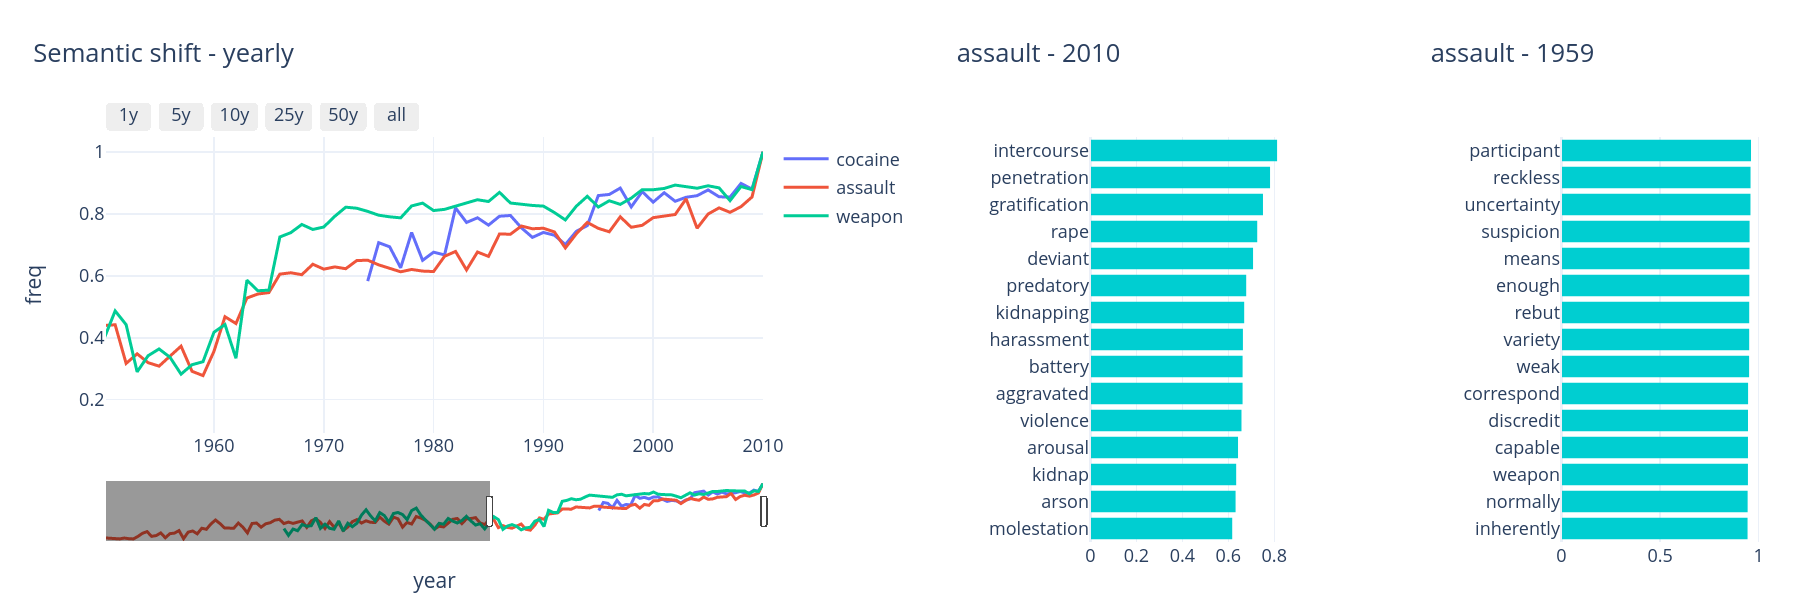
\includegraphics[width=\textwidth]{images/semantic_2.png}
  \caption{Semantic shift of the word cocaine, assault and weapon 
  with respect to the year 2010. A drop of the assault curve in 1959 correspond to 
  a different context with respect to the base year, as proven by the different similar words.} \label{fig2}
\end{center}
\end{figure}

\begin{figure}
  \begin{center}
    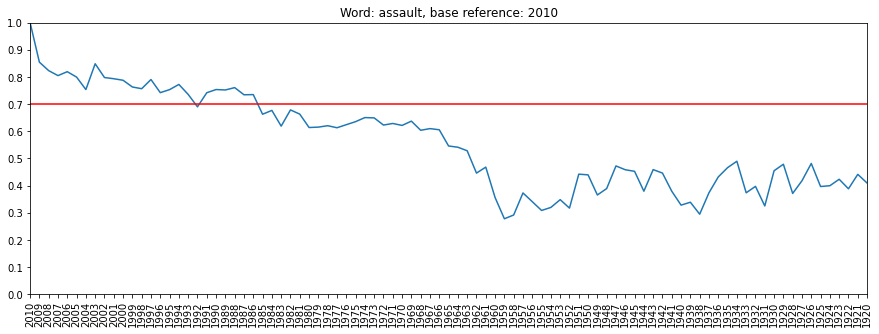
\includegraphics[width=\textwidth]{images/semantic_1.png}
    \caption{Similarity between consecutive epochs of the terms cocaine, assault and weapon. Comparing 
    the similar words, we can see that the drop of the cocaine curve around 1970 correspond to a shift in context.} \label{fig3}
  \end{center}
\end{figure}

\subsection{Webapp}
In order to visualize and explore the results of the analysis, a web interface has been developed. Through the UI, the
user can search multiple words united, separated by ",", and/or compare words, separated by "-"; the app will show
various interesting sections, one focused on the analysis of the searched words: 
% an example can be seen on figure
% \vref{fig4}, and one on the
% analysis of a selected topic, figure \vref{fig5}:
\begin{itemize}
  \item Top 15 words of similar context of the searched words, using word embeddings.
  \item Frequency graph of documents in time containing the searched words.
  \item Semantic shifts of the searched words, both by epoch, two adjacent epochs of 10 years, and by single year.
    If the user clicks on a point of the graph, the contexts of the selected word in the different selected years/epochs
    will be showed, allowing the comparison of contexts which helps understanding the evolution of words meaning and usage
    during time.
  \item Topic distribution of the searched words, both generic and areas of interest-specific topics. By clicking on the
    showed radar chart, or on the lateral list of topics, the selected topic info will be loaded in the below section.
  \item Most important words of the selected topic. There are three ways of visualization: a barchart with the first 15
    words, a Wordcloud with the first 80 and a Treemap with the first 50.
  \item Topic distribution over time and over the different Illinois courts.
\end{itemize}

\subsubsection{Webapp developing technology}\hfill\\

In order to fastly create an interesting interface, three python-based frameworks for web developing have been considered:
\begin{itemize}
    \item Voila and ipywidgets. Because the whole project has been developed using Jupyter notebooks, it would have
    been natural to develop the webapp in a new notebook. ipywidgets allow to create dynamic elements and behaviour to
    a Jupyter Notebook, while Voila allows to have better design and the possibility to run the notebook as if it is
    a web page, hiding all the code and markdown of the notebook itself.
    \item Dash. It consists in a point-\&-click interface to models written in Python, vastly expanding the notion of
    what's possible in a traditional "dashboard." It is the main solution for data scientists and engineers in order to
    put complex Python analytics in the hands of business decision-makers and operators.
    \item Streamlit. Similar to Dash.
\end{itemize}
Voila and ipywidgets have been discarded because of the technical requirements needed to run and understand a Jupyter
notebook; even if the complexity could have been partially hidden, the graphics component of ipywidgets are not so
captivating.

Dash and Streamlit are really similar one to another, with both offering beautiful interfaces easy to deploy. Dash has
been chosen because of its popularity and presence in the data science applications world, but Streamlit is quite new
but in the last years it has gained a lot of popularity and attention.

In all three frameworks, and particularly in Dash, the workflow is pretty similar; the design elements of the UI are
defined in an HTML-style using the framework Python libraries predefined classes, while the user-generated events are
captured using callback functions, which connect the input elements (e.g. a button which has been clicked) to output
elements (e.g. a graph), defining the required processing and manipulation of output elements.

\subsubsection{Cloud hosting}\hfill\\

Since the developed webapp prototype shows some potential in finding interesting trends about words, we 
decided to host the project on a public domain, in order to give anyone the possibility to make queries 
without a technical knowledge or any installation requirement.

Firstly, many free-to-use hosting sites of Python web applications have been tested, such as PythonAnywhere and Heroku,
but all of them allowed a to small free tier, for instance of one gigabyte of disk. 
Because of the large data that is used to show the various statistics, having models taking up to five gigabytes of space,
it was not possible to use any of them.

Google Cloud Platform has been chosen to host the webapp. A Docker image of the project has been created, which
has been built to Google Cloud Run, creating an online container of 16GB of memory and 4 CPUs, the last and only combination allowed which permitted also to load all the
required files. 
Google Cloud offers a huge Free Tier, but because of the demanding configuration,
the monthly cost is expected to be around three dollars.
One downside of the selected hosting method is that the container instance is active only during the
period in which requests are served, thus, if no other instance is active, the container has to be launched
from an idle state, taking about three or four minutes to be accessible, due to the amount of files that it
has to load in order to make all the analysis functionality available.

\subsection{Interesting findings}
\label{sec:Interesting findings}

We now present a collection of interesting findings with the developed tools.
The webapp allows to search for single or combinations of words, and the data on context change and topics can 
reveal really interesting trends in time. 

The first one is about murders, in particular the difference of context between murders involving men and 
women. In the first case, the topics associated with the combination murder-man are theft related, while in the 
second case, murder-woman is associated with the sexual victims topic. Searching for murder and rape reveals 
similarity with kidnaps and robberies. 

A second finding is about the context change of the word drug, in fact, the ten year epoch similarity 
drops between 1940 and 1950, in the first case the word is associated with groceries, while in the 
second the word shifted towards a narcotic context.

If we associate the words drug and death we find that overdose is the closets word in term of vector distance.

Another example is the change of context of the word homosexual, in the 60s it is associated with words such as 
deviate, aggressive, unnatural, while in modern times it refers to sexual orientation.

Analyzing the word assault, we can see that in the 60s it was associated with armed crimes, 
while in modern days it has a sexual crime context. 

In the most similar words with respect to home and murder combined we can find boyfriend, girlfriend and fiance.

Regarding courts and topics, we can 